
%\section{Analisi di mercato}
\section{Metarace}

    Metarace è un progetto in Unreal Engine che punta a sfruttare i dispositivi AR/VR per far immergere l'utente in un mondo virtuale di competizioni equestri.
    %
    Si definisce un progetto nel Metaverso perché punta ad avere le caratteristiche che definiscono tutte le piattaforme attualmente vicine a questo concetto: una rappresentazione digitale della persona sotto forma di avatar, un ambiente virtuale in cui è possibile interagire e socializzare con altri utenti, degli oggetti di gioco personalizzabili e portabili al di fuori di Metarace, un'economia interna e una progettazione focalizzata sulla scalabilità per permettere in futuro di aggiornare l'applicativo all'arrivo di nuove tecnologie.
    %
    In Metarace il giocatore può possedere dei cavalli virtuali e li può iscrivere a delle competizioni in cui competono con i cavalli di altri giocatori.
    %
    Il giocatore può assistere alle competizioni con un avatar virtuale entrando nel mondo attraverso un visore per la realtà virtuale. 
    %
    In mancanza di questo può comunque assistere alla gara tramite desktop. 
    %
    Il vincitore di ogni gara sarà determinato da una componente intrinseca al cavallo in termini di forza innata e una componente randomica relativa alla singola gara.

    L'idea dietro al gioco è quella di far immergere l'utente in un ambiente simile a quello delle competizioni equestri che si svolgono nel mondo reale, dove quindi gli spettatori e i proprietari dei cavalli non prendono parte attiva alla competizione ma vi assistono dagli spalti e dove la vittoria non è mai certa. 
    %
    L'idea di Metarace è di riproporre questa formula in un ambiente virtuale immersivo, nel Metaverso.

\section{La meccanica di base} \label{sec:Meccanica}

    Una partita di Metarace consiste in una gara di cavalli in cui c'è sempre un vincitore, con una piccola probabilità di pareggio.
    %
    Il risvolto della gara è dato da caratteristiche intrinseche dei cavalli gareggianti e da fattori casuali.

    Siccome il giocatore non prende parte attiva alla gara ma vi assiste attraverso il proprio avatar, l'esito della gara è deciso da un server che invia il risultato a ciascun client dei partecipanti.
    %
    Il client calcola, attraverso un algoritmo, il comportamente dei cavalli in modo che sia coerente con il risvolto della gara inviato dal server.
    %
    Il server invia al client un insieme di array di tempi.
    %
    Il client divide il percorso in un numero di step uguale alla cardinalità di questi array e poi fa percorrere ai cavalli questi step sulla base dei tempi stessi.
    %
    Il client perciò si occupa di renderizzare il mondo di gioco, di far iscrivere l'utente alle competizioni che desidera e a consentire la fruizione della gara.
    %
    Durante lo sviluppo, è stata trovata subito la necessità di testare come poter tradurre questi dati inviati dal server in movimenti dei gareggianti all'interno del mondo di gioco.

    \subsection{L'algoritmo per il movimento dei cavalli}

        Lo strumento più adatto tra quelli messi a disposizione da Unreal Engine per implementare questa meccanica è la Spline Component.
        %
        Una Spline Component è un percorso che lo sviluppatore può definire per utilizzare dati posizionali.
        %
        Può essere usata per far muovere oggetti o per posizionare una serie di Actor lungo di essa.
        %
        Questo componente è composto da una serie di nodi ordinati, posizionabili all'interno del mondo di gioco, e da una linea che segue questi nodi in maniera interpolata andando a creare così il percorso.
        %
        È inoltre possibile far seguire una Spline ad una Mesh (o ad un Actor) impostando un'animazione basata sul tempo.
        %
        Questo in Unreal è possibile farlo attraverso una Timeline.
        %
        Una Timeline è uno strumento offerto da Unreal Engine che permette di ottenere dei valori di output nel tempo basati su una Curve impostata inizialmente.

        Quello che ho implementato è stato di creare una classe C++ che rappresenta il cavallo e un Blueprint che la estendeva.
        %
        Inoltre ho creato un altro Blueprint che contiene tutte le Spline del percorso.
        %
        Ogni cavallo sarà associato ad una delle Spline e la seguirà secongo l'algoritmo seguente:

        \begin{lstlisting}[caption = Sezione del file header (movimento cavallo)]
FTimeline RaceTimeline;
UPROPERTY()
USplineComponent* SplineComponent = nullptr;
UPROPERTY()
UCurveFloat* CurveFloat;
        \end{lstlisting}

        La Timeline si utilizza attraverso una funzione che ne cattura il progresso (legata con una \textit{FOnTimelineFloat}) e grazie ad una \textit{CurveFloat} che ne definisce il comportamento. 
        %
        Per legare un oggetto \textit{FOnTimelineFloat} alla funzione per catturare l'output della Timeline si utilizza la funzione \textit{BindUFunction}.
        %
        Per associare la Timeline alla \textit{FOnTimelineFloat} e alla \textit{CurveFloat} si utilizza la funzione \textit{AddInterpFloat} chiamata dalla Timeline stessa.

        \begin{lstlisting}[caption = Inizializzazione della Timeline nel file source (movimento cavallo)]

void AHorse::Inizialize()
{
    [...] //creazione della CurveFloat

    FOnTimelineFloat RaceTimelineProgress;
    RaceTimelineProgress.BindUFunction(
        this, FName("RaceTimelineProgress"));
    if(RaceCurveFloat){ //per evitare nullptr exception
        RaceTimeline.AddInterpFloat(
            RaceCurveFloat, RaceTimelineProgress);
    }
    [...] // Settaggio del RatePlay della Timeline 
}

        \end{lstlisting}

        Per far partire la Timeline bisogna chiamare la funzione \textit{Play()}.

        \begin{lstlisting}
void AHorse::StartTimeline()
{
    RaceTimeline.Play();
}\end{lstlisting}

        Il valore di output della Timeline (che ho chiamato \textit{Value}) è standardizzato tra 0 e 1.
        %
        È possibile eseguire un interpolazione tra 0 e la lunghezza della Spline basata su questo valore e ottenere così una posizione lungo la Spline.
        %
        La posizione dell'Actor viene quindi impostata uguale alla posizione trovata.

        \begin{lstlisting}[caption = Funzione che sfrutta il valore restituito dalla timeline nel tempo  (movimento cavallo)]
void AHorse::RaceTimelineProgress(float Value)
{    
    if(MeshComponent && SplineComponent)
    {
        float DistanceInSpline = FMath::Lerp(0, 
            SplineComponent->GetSplineLength(), 
            Value);
        FTransform TransformAtDistance = 
            SplineComponent->GetTransformAtDistanceAlongSpline(
                DistanceInSpline, 
                ESplineCoordinateSpace::World);
        SetActorLocationAndRotation(
            TransformAtDistance.GetLocation(),
             TransformAtDistance.GetRotation());
    }
}
        \end{lstlisting}

        Questa funzione viene chiamata automaticamente dalla Timeline se all'interno della funzione \textit{Tick} le viene passato il valore \textit{DeltaTime}.
        %
        La funzione \textit{Tick} è chiamata automaticamente da Unreal Engine ad ogni frame e il valore \textit{DeltaTime} è il tempo che è intercorso dall'ultima chiamata della funzione \textit{Tick} (equivalente al tempo intercorso dall'ultimo frame).

        \begin{lstlisting}[caption = Funzione Tick (movimento cavallo)]
void AHorse::Tick(float DeltaTime)
{
    Super::Tick(DeltaTime);

    RaceTimeline.TickTimeline(DeltaTime);
}
        \end{lstlisting}

        Per far muovere la Mesh Component coerentemente all'array di tempi inviato dal server, bisogna creare una \textit{FloatCurve} che si basa su di essi.
        %
        Questo viene fatto nella funzione \textit{Inizialize}.
        %
        La classe \textit{UCurveFloat} non offre funzioni che permettono di instanziarne una a tempo di esecuzione, per questo viene utilizzata una \textit{FRichCurve} per la sua creazione runtime.
        %
        Sia la \textit{FRichCurve} che la \textit{CurveFloat} sono costituite da una serie di punti su un piano cartesiano e hanno entrambe delle regole di interpolazione da un punto ad un altro.
        %
        Le regole per la definizione dell'interpolazione si possono definire grazie alla struct \textit{ERichCurveInterpMode} che può essere: \textit{RCIM\_Linear} (interpolazione lineare), \textit{RCIM\_Cubic} (interpolazione cubica) oppure \textit{RCIM\_None} (nessuna interpolazione).
        %
        Si inizia con la definizione di variabili temporanee per lo spazio e il tempo, si definisce inoltre la lunghezza standardizzata di ogni step sulla curva e si calcola il tempo totale che il cavallo impiegherà a percorrere tutto il percorso:

        \begin{lstlisting}[caption = Definizione variabili temporanee (movimento cavallo)]
void AHorse::Inizialize()
{
    float TempS = 0; //Variabile temporanea per lo Spazio
    float TempT = 0; //Variabile temporanea per il Tempo
    
    //Lunghezza di ogni step standardizzata 
    float DeltaS = 1 / float(TimeArray.Num());
    
    for(float Time : TimeArray)
    {
        //Tempo complessivo per percorrere tutto il percorso
        TotalTime += Time;
    }
        \end{lstlisting}

        Una volta definite queste variabili si inizia la creazione della curva.
        %
        Il numero dei punti sul piano cartesiano equivale al numero degli elementi dell'array dei tempi più un punto iniziale all'origine del piano cartesiano.
        %
        Un'istanza della classe \textit{FRichCurve} è costituita da una serie di \textit{FRichCurveKey}, perciò popolo un \textit{TArray} con delle keys di questo tipo.
        %

        \begin{lstlisting}[firstnumber=15]
    RichCurve = new FRichCurve();

    TArray<FRichCurveKey> Keys;
    FRichCurveKey FirstKey = FRichCurveKey(0, 0, 0, 1, 
        ERichCurveInterpMode::RCIM_Cubic);
    Keys.Add(FirstKey);
        \end{lstlisting}

        Per la creazione delle keys itero su tutti gli elementi dell'array di tempi e ad ogni iterazione sommo il tempo \textit{i} con la somma di tutti i tempi precedenti diviso la somma di tutti i tempi in modo da ottenere un valore standardizzato.
        %
        Ossia ogni key ha come variabile tempo:

        \begin{equation}
            T_{i = 0..n} = \sum^{i}_{j = 0} \frac{t_j}{t_{tot}}
        \end{equation}

        Ogni key ha come variabile spazio la lunghezza standardizzata del singolo step moltiplicato il numero di iterazione corrente:

        \begin{equation}
            S_{i = 0..n} =  \Delta S (i+1)
        \end{equation}

        Inoltre l'ultima key generata non ha interpolazione per evitare che i cavalli prima dell'arrivo inizino a rallentare.

        \begin{lstlisting}[firstnumber=22]
    for (int i = 0; i<TimeArray.Num(); i++)
    {
        TempS = DeltaS * (i + 1);							
        TempT += TimeArray[i] / TotalTime;
        FRichCurveKey Key;
        if((i+1) < TimeArray.Num())
        {
            Key = FRichCurveKey(TempT, TempS, 0, 0,
                ERichCurveInterpMode::RCIM_Cubic);
        }
        else
        {
            Key = FRichCurveKey(TempT, TempS, 1, 0, 
                ERichCurveInterpMode::RCIM_None);
        }
        Keys.Add(Key);
    }
        \end{lstlisting}

        Una volta generate le keys le aggiungo alla \textit{FRichCurve}, poi istanzio un nuovo oggetto \textit{UCurveFloat} e setto le sue keys essere quelle della \textit{FRichCurve}.

        \begin{lstlisting}[firstnumber=40]
    RichCurve->SetKeys(Keys);
    UCurveFloat* RaceCurveFloat = NewObject<UCurveFloat>();;
    RaceCurveFloat->FloatCurve = *RichCurve;

    [...] // Inizializzazione della Timeline
        \end{lstlisting}

        Infine imposto il RatePlay della Timeline uguale alla frequenza con cui il cavallo si muove lungo il percorso.

        \begin{lstlisting}[firstnumber=46]
    RaceTimeline.SetPlayRate(1 / TotalTime);	
}
        \end{lstlisting}

        % Ne devi cercare un'altra questa sembra troppo una linea
        \begin{figure}[!ht]
            \centering
            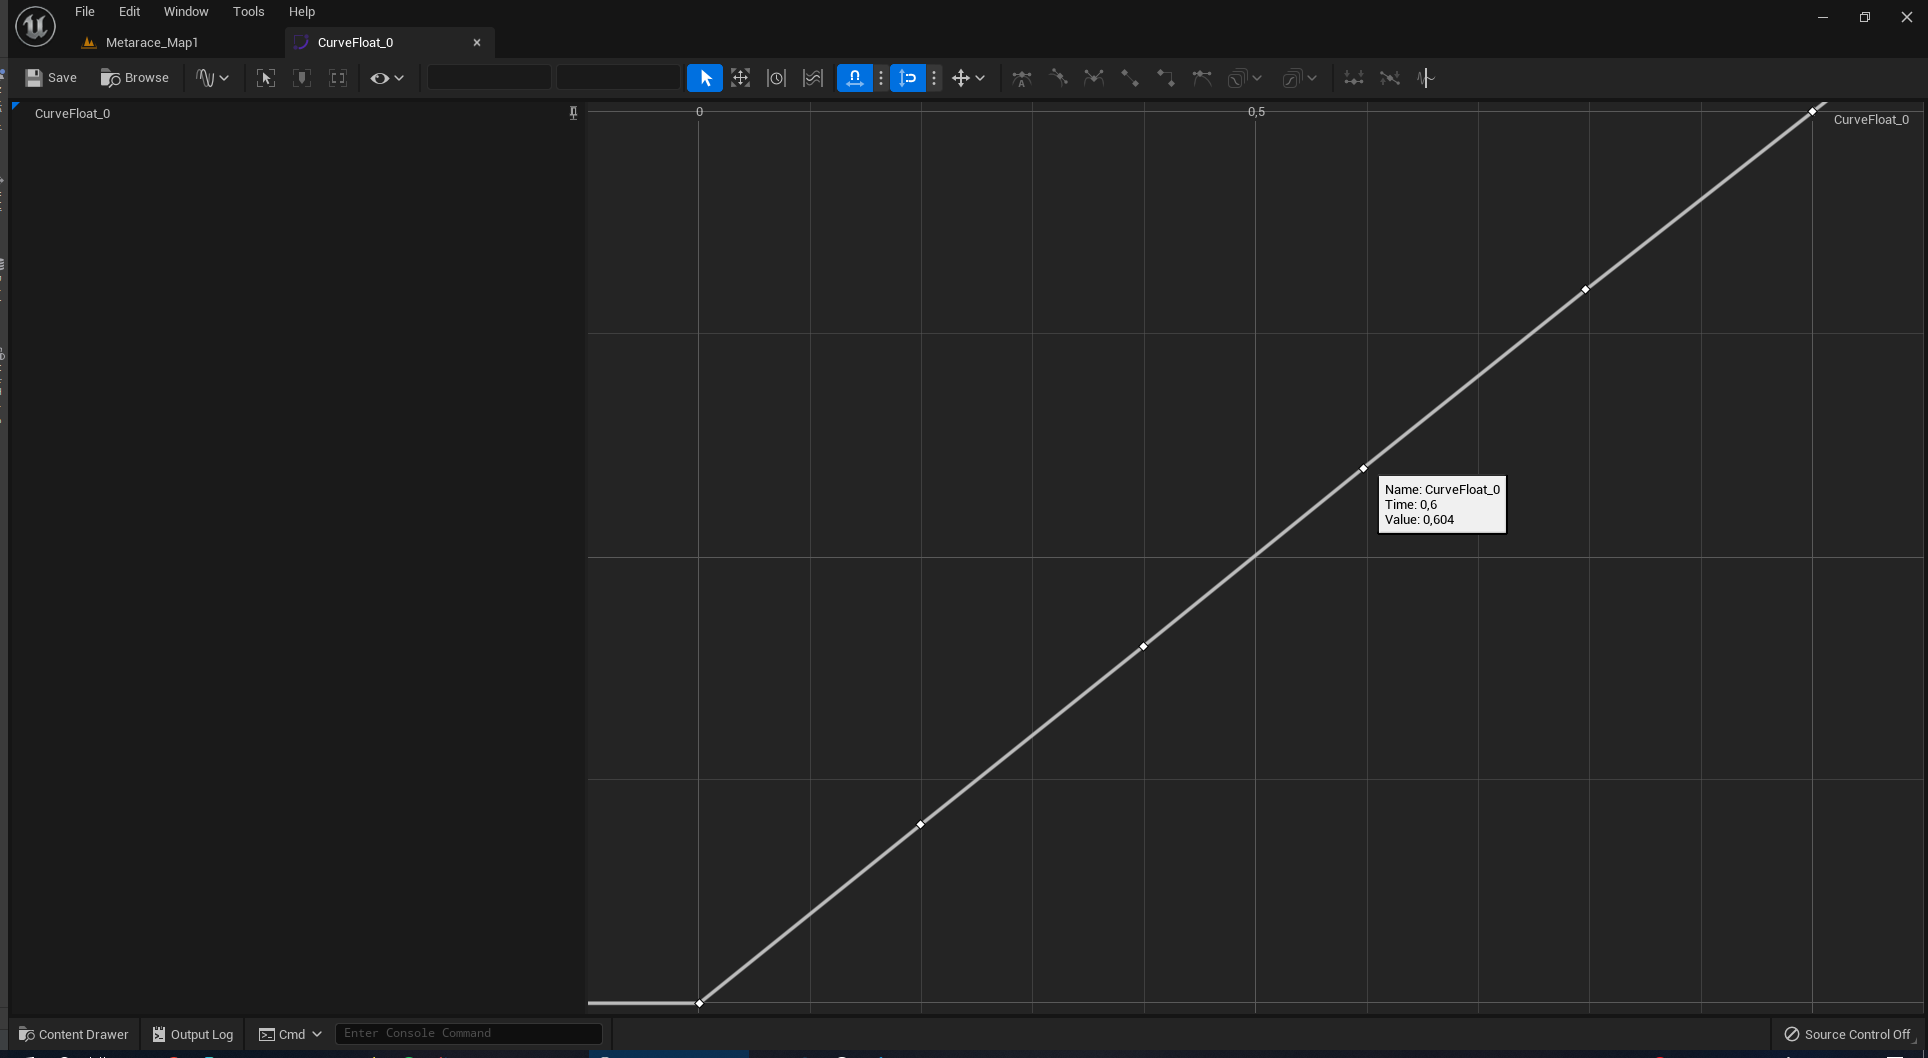
\includegraphics[width=10cm]{figure/FloatCurve.png}
            \caption{\textit{UCurveFloat} generata dall'algoritmo per il movimento dei cavalli}
            \label{fig:CurveFloat}
        \end{figure}

        Questo processo genera una curva come quella mostrada in Figura \ref{fig:CurveFloat}.
        %
        Questa curva garantisce un cambiamento di velocità fluido del cavallo durante tutta la gara nonostante, dall'immagine, i cambiamenti di coefficiente angolare non siano apprezzabili.

    \section{Animazione dei cavalli}

    I cavalli non soltanto si muovono lungo il percorso ma possiedono una serie di animazioni che vengono riprodotte in base allo stato in cui si trovano e alla velocità che possiedono.
    %
    I cavalli infatti sono delle Mesh associate ad uno scheletro gerarchico di ossa che può essere animato per muovere la Mesh.
    %
    Questo tipo di Mesh vengono gestite con Unreal Engine come delle Skeletal Mesh. 
    %
    Per la gestione delle animazioni in Unreal Engine si può utilizzare uno strumento chiamato \textit{AnimGraph}.
    %
    Questo strumento valuta la pose da mostrare per una Skeletal Mesh in ogni frame in base alle animazioni passate come input \cite{UAnimGraph}.

    \begin{figure}[!ht]
        \centering
        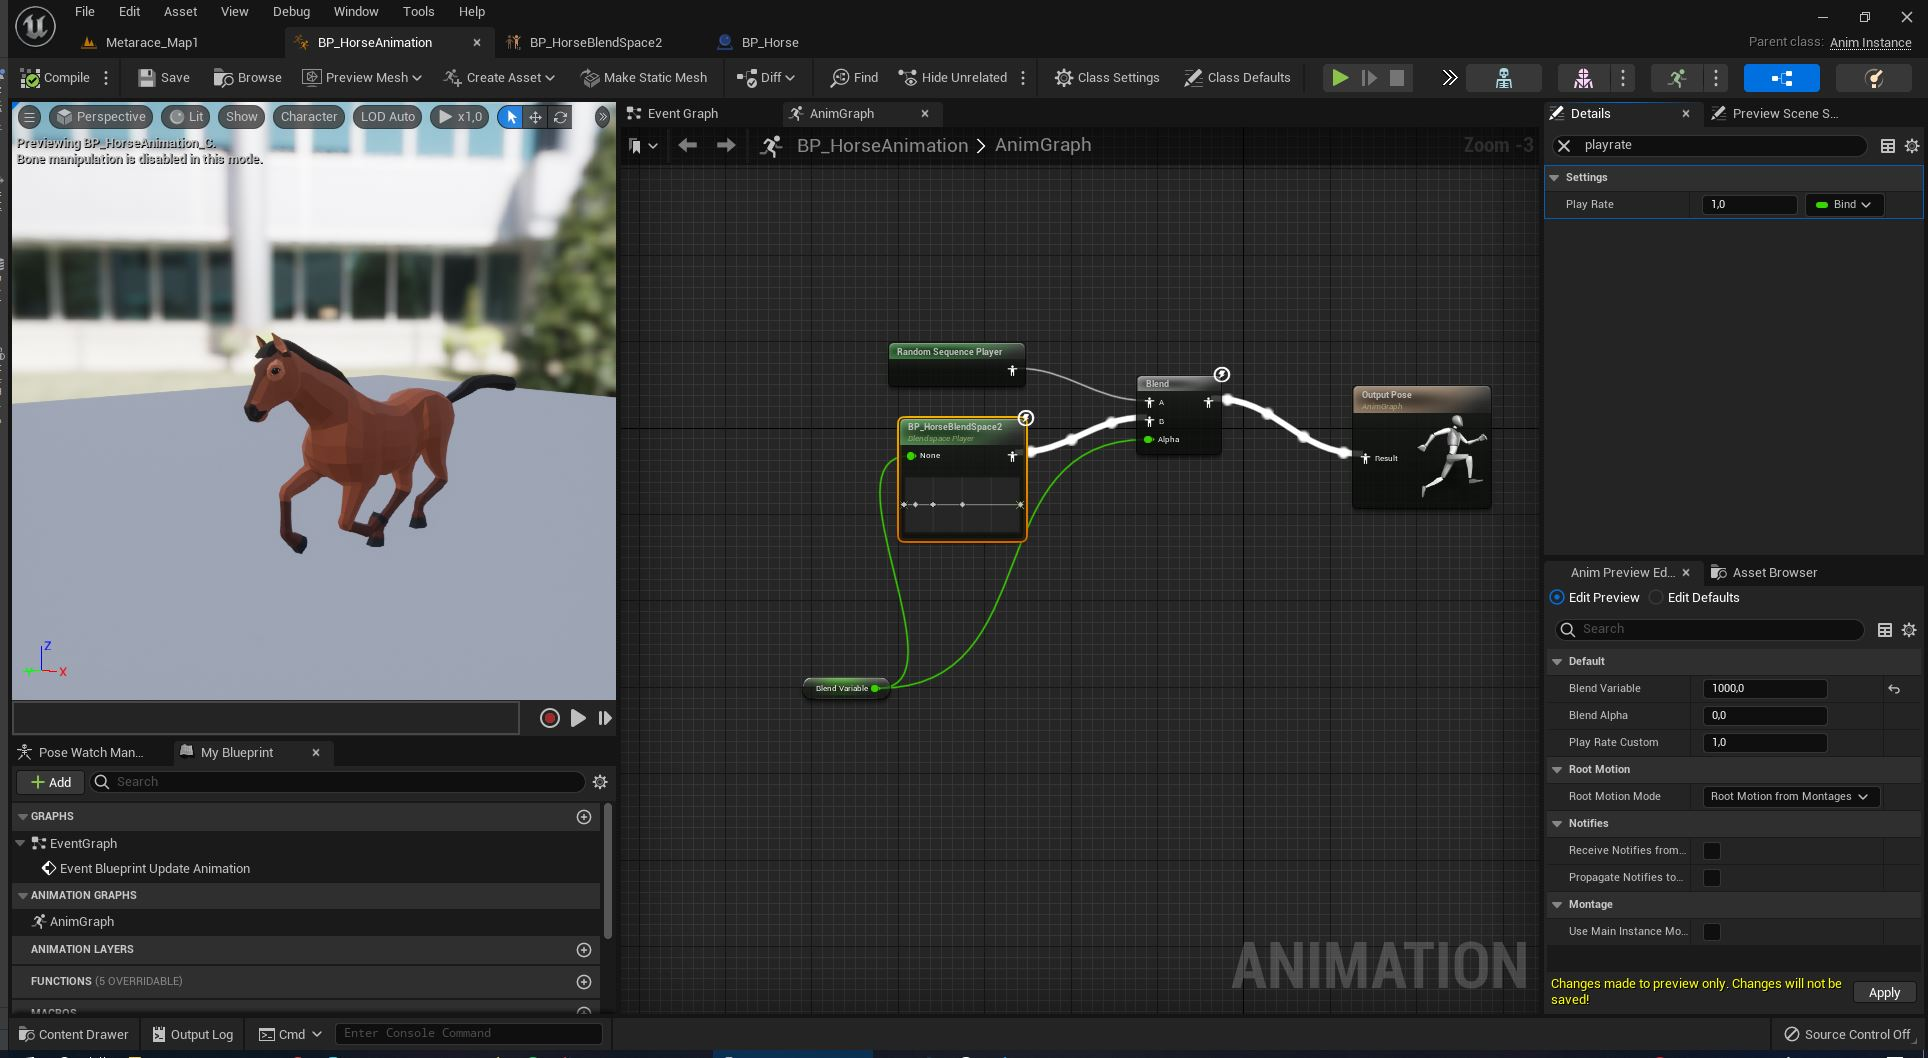
\includegraphics[height=7cm]{figure/HorseAnimGraph.JPG}
        \caption{\textit{AnimGraph} che gestisce l'animazione del cavallo.}
        \label{fig:AnimGraph}
    \end{figure}

    L' \textit{AnimGraph} mostrato in Figura \ref{fig:AnimGraph} utilizza due lettori di animazione: un \textit{BlendSpace2D} e un \textit{Random Sequence Player}.
    
    Il \textit{Random Sequence Player} è un lettore che permette di salvare una lista di animazioni da riprodurre.
    %
    Queste animazioni vengono riprodotte in maniera casuale una dopo l'altra.
    %
    Questo nodo è perfetto per riprodurre le animazioni \textit{Idle} del cavallo (le animazioni per quando il cavallo è fermo).

    Il \textit{BlendSpace2D} invece è un asset speciale che permette di fare il blend tra più animazioni sulla base di un valore in input.
    %
    Per sfruttarlo bisogna inserire le animazioni lungo l'asse delle ascisse che il nodo mostra.
    %
    Posizionando le animazioni in maniera adeguata, ossia per far combaciare il valore di input con la frequenza di riproduzione delle animazioni, si ottiene un blend automatico tra le animazioni legato al valore di input.
    %
    L'editor aiuta in questo processo segnalando un errore quando l'animazione non combacia con il valore sull'asse.
    %
    In questo contesto è stato utilizzato come valore di input la velocità del cavallo e questo fa si che ognuno di questi possiede, in ogni momento, un'animazione coerente con l'andatura che mantiene.
    %
    Questa tecnica risolve il problema del "pattinamento" - ossia quando un'animazione è più lenta o più veloce di quanto un Actor si muova in scena avendo come effetto quello di sembrare che scivoli (che appunto pattini) sul terreno - nonostante le animazioni date in input non sarebbero adeguate per la velocità sostenuta.
    %
    Questo perché l'animazione risultante è in realtà un'interpolazione delle animazioni di input in base, appunto, alla velocità.
    %
    Le animazioni inserite in questo BlendSpace sono 4: una di \textit{Idle}, una di camminata, una per il trotto, una per la corsa leggera e una per il galoppo.

    \begin{figure}[!ht]
        \centering
        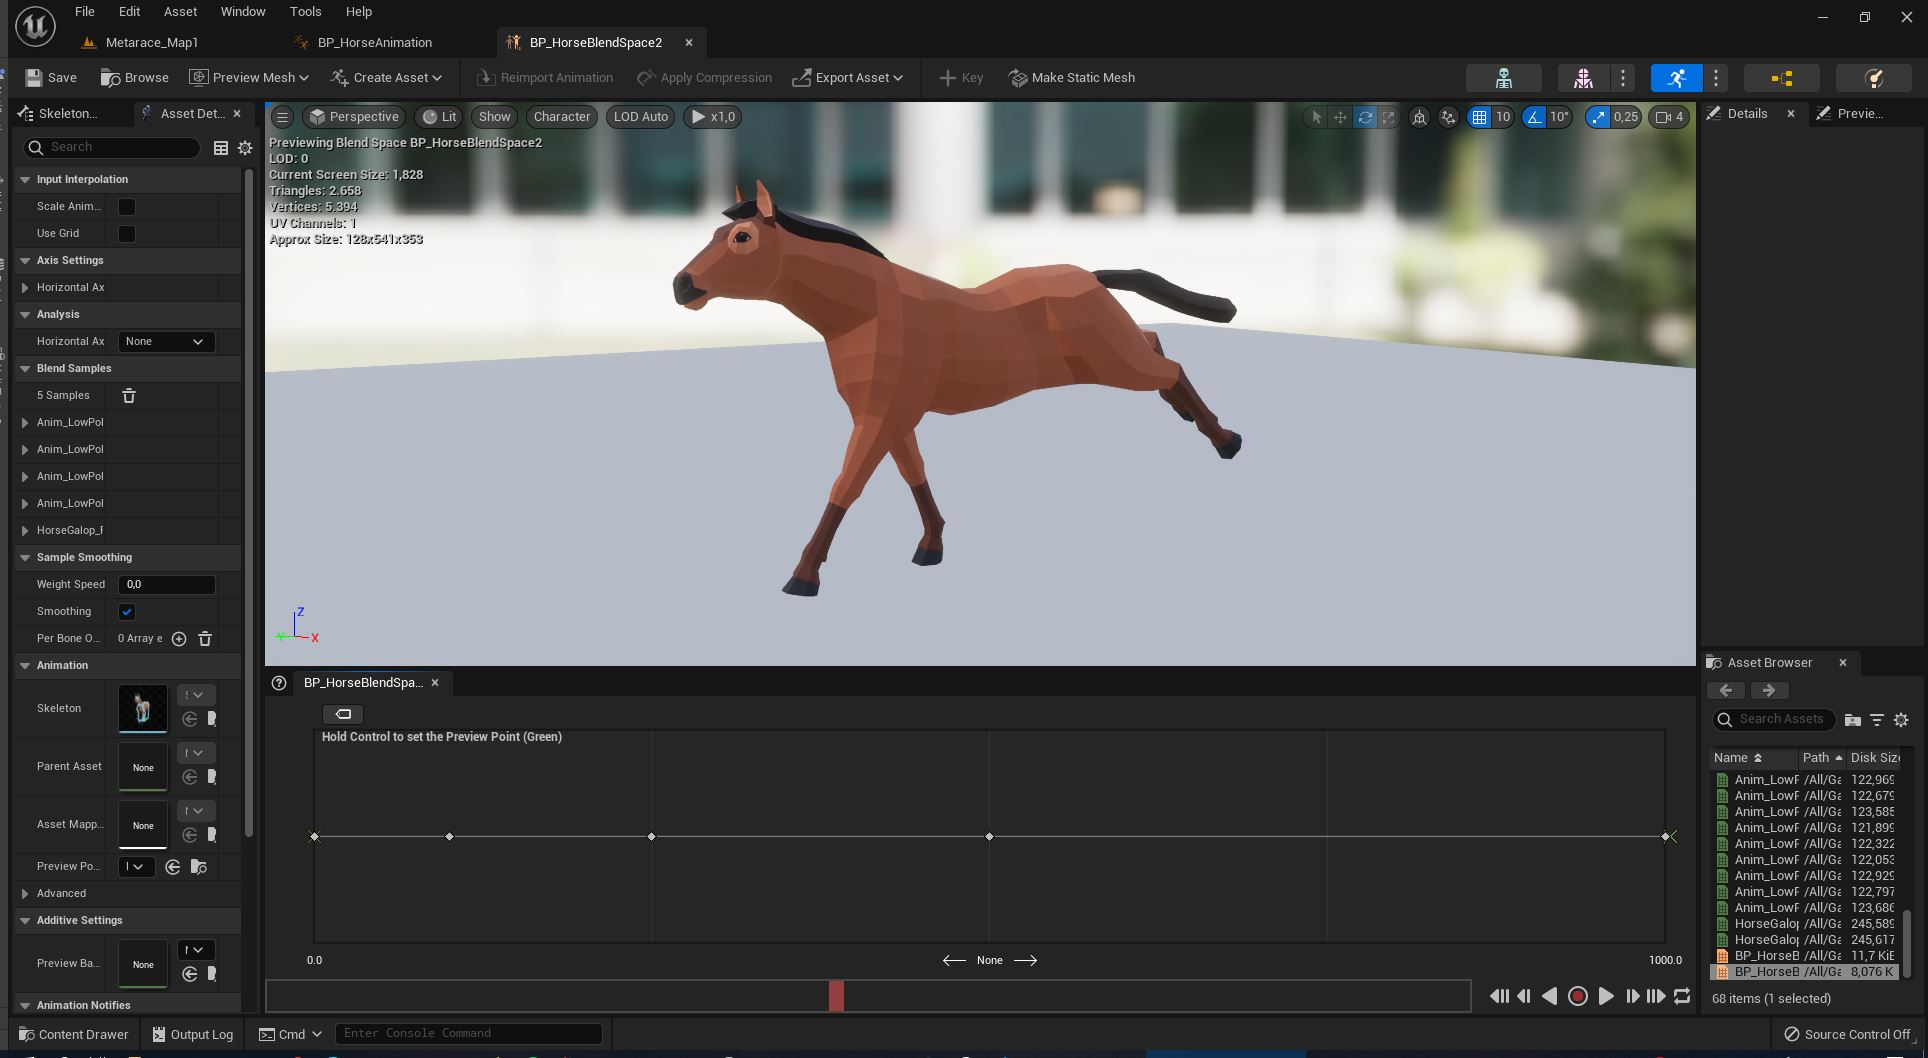
\includegraphics[height=7cm]{figure/HorseBlendSpaceGalop.JPG}
        \caption{\textit{BlandSpace2D} per l'interpolazione delle animazioni sulla base della velocità.}
    \end{figure}

    Come si può vedere dalla Figura \ref{fig:AnimGraph}, il valore di input per il BlandSpace è utilizzato anche come valore di blend tra il \textit{BlendSpace2D} e il \textit{Random Sequence Player}.
    %
    Questo perché quando il valore di input è nullo vuol dire che si è raggiunta l'andatura in cui è possibile riprodurre una tra le animazioni di \textit{Idle} e perciò ne viene riprodotta una casualmente. 

    \subsection{Animazione del galoppo creata con Blender}

    Un cavallo non può considerarsi un cavallo da corsa senza un'animazione del galoppo.
    %
    Per questo motivo ho ideato e creato l'animazione in questione nella suite Blender.

    La suite Blender permette di animare qualsiasi tipo di oggetto e qualsiasi tipo di deformazione o traslazione tramite la tecnica di inserimento di \textit{keyframe poses} all'interno di una finestra apposita: l'Action Editor. 
    %
    Letteralmente keyframe pose vuol dire "posa del fotogramma chiave", questo perché questa tecnica prevede di salvare tutti i dati sul Transform (quindi su posizione, rotazione e scala) di uno o più oggetti all'interno di vari frame che riprodotti in sequenza andranno a creare l'effetto di movimento che compone l'animazione.
    %
    Questa tecnica è particolamente efficace per le mesh associate ad uno scheletro gerarchico di ossa (chiamato rig).
    %
    Infatti muovendo una o più ossa si andrà a deformare la mesh senza cambiarne la geometria ma solo cambiandole la posizione, creando una pose, e salvando queste pose nelle keyframe si potrà salvare ed esportare la riproduzione delle keyframe come un'animazione.

    \begin{figure}[!ht]
        \centering
        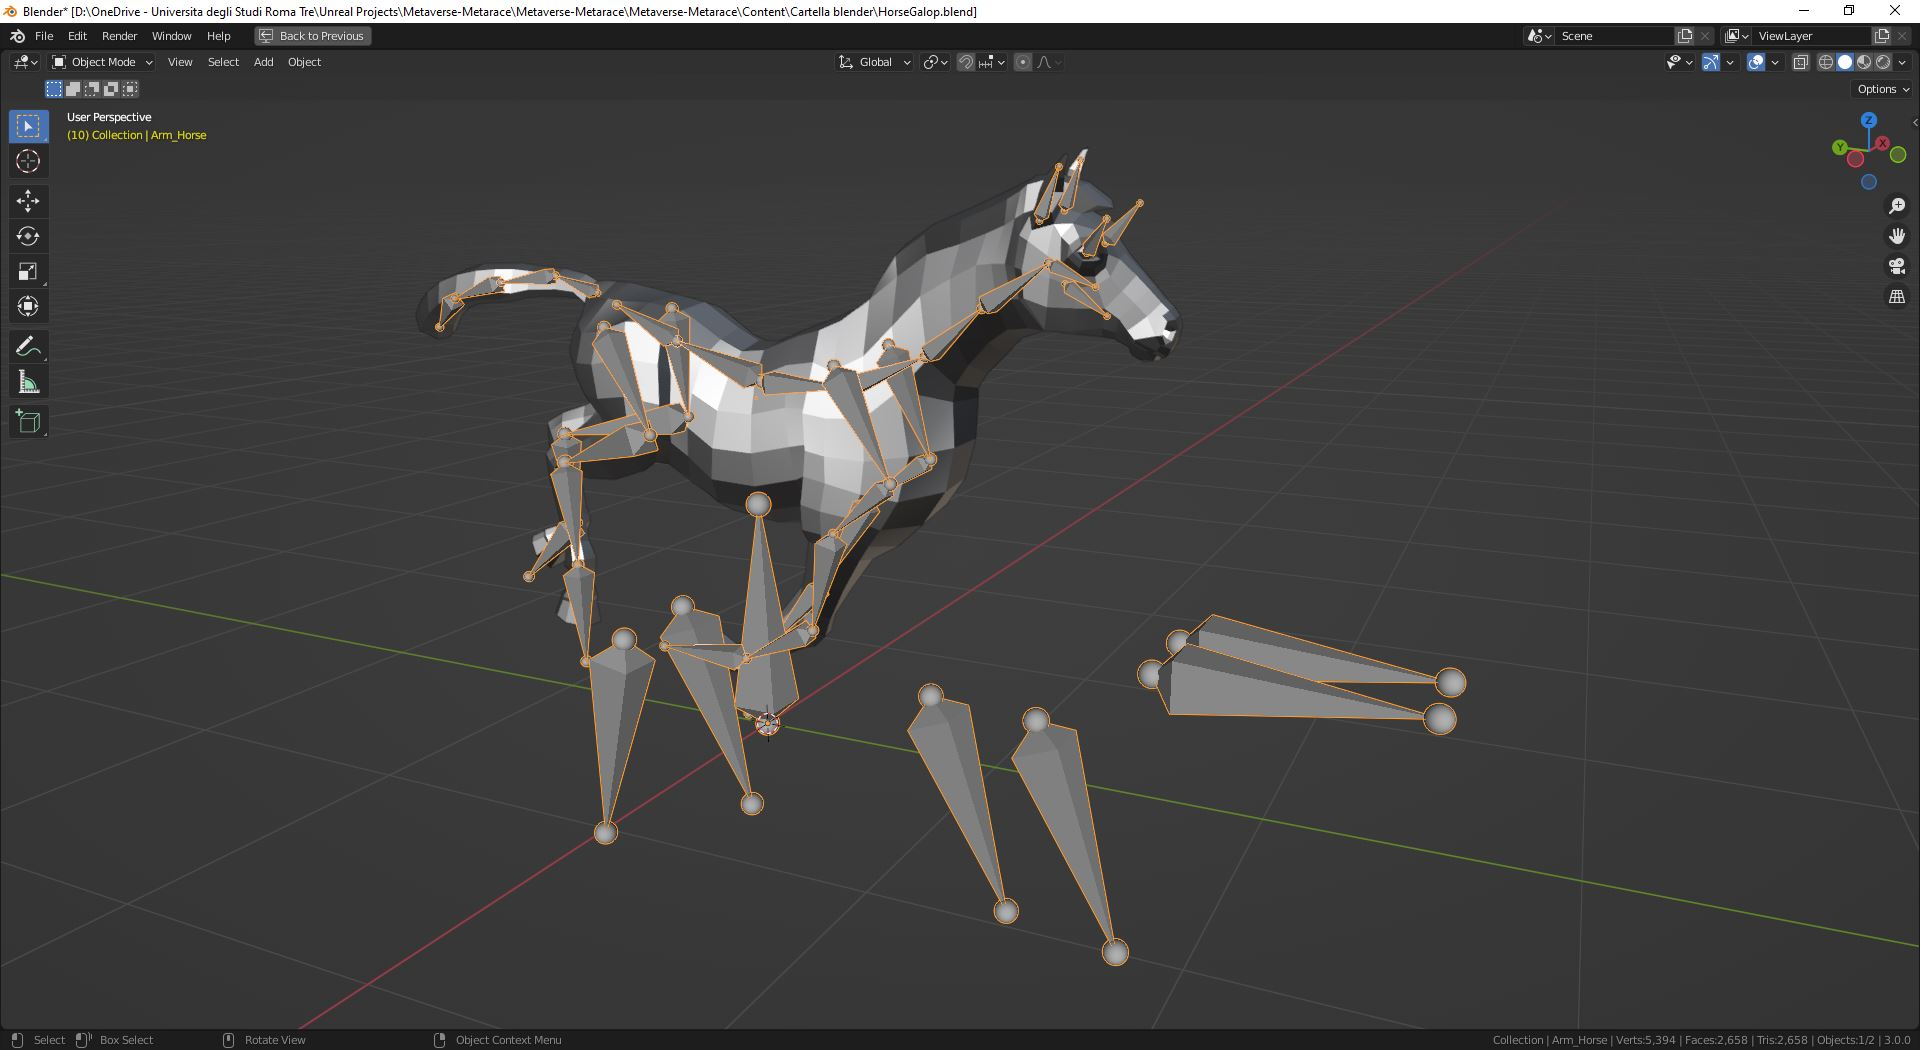
\includegraphics[width=10cm]{figure/HorseRig.JPG}
        \caption{Vista in Blender della Mesh del cavallo, con il suo rig associato, in una pose tra le 12 dell'animazione del galoppo}
    \end{figure}

    Creare animazioni convincenti è un'arte molto complessa che va studiata a fondo.
    %
    Spesso il modo migliore per crearne una è partire da una reference del mondo reale e così ho fatto.
    %
    Sono partito da un'immagine che rappresenta lo studio alla base dell'animazione del galoppo diviso in 12 frame e ho cercato di far combaciare la posizione della mesh con quella che si vede nell'immagine per ogni singolo frame.

    \begin{figure}[!ht]
        \centering
        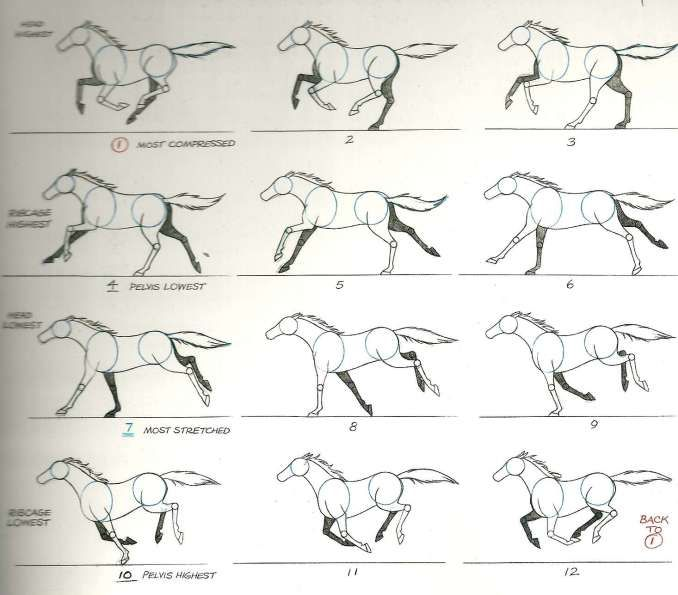
\includegraphics[height=6.5cm]{figure/HorseAnimation.jpg}
        \caption{12 frame disegnati di un cavallo al galoppo}
    \end{figure}

    \begin{figure}[!ht]
        \centering
        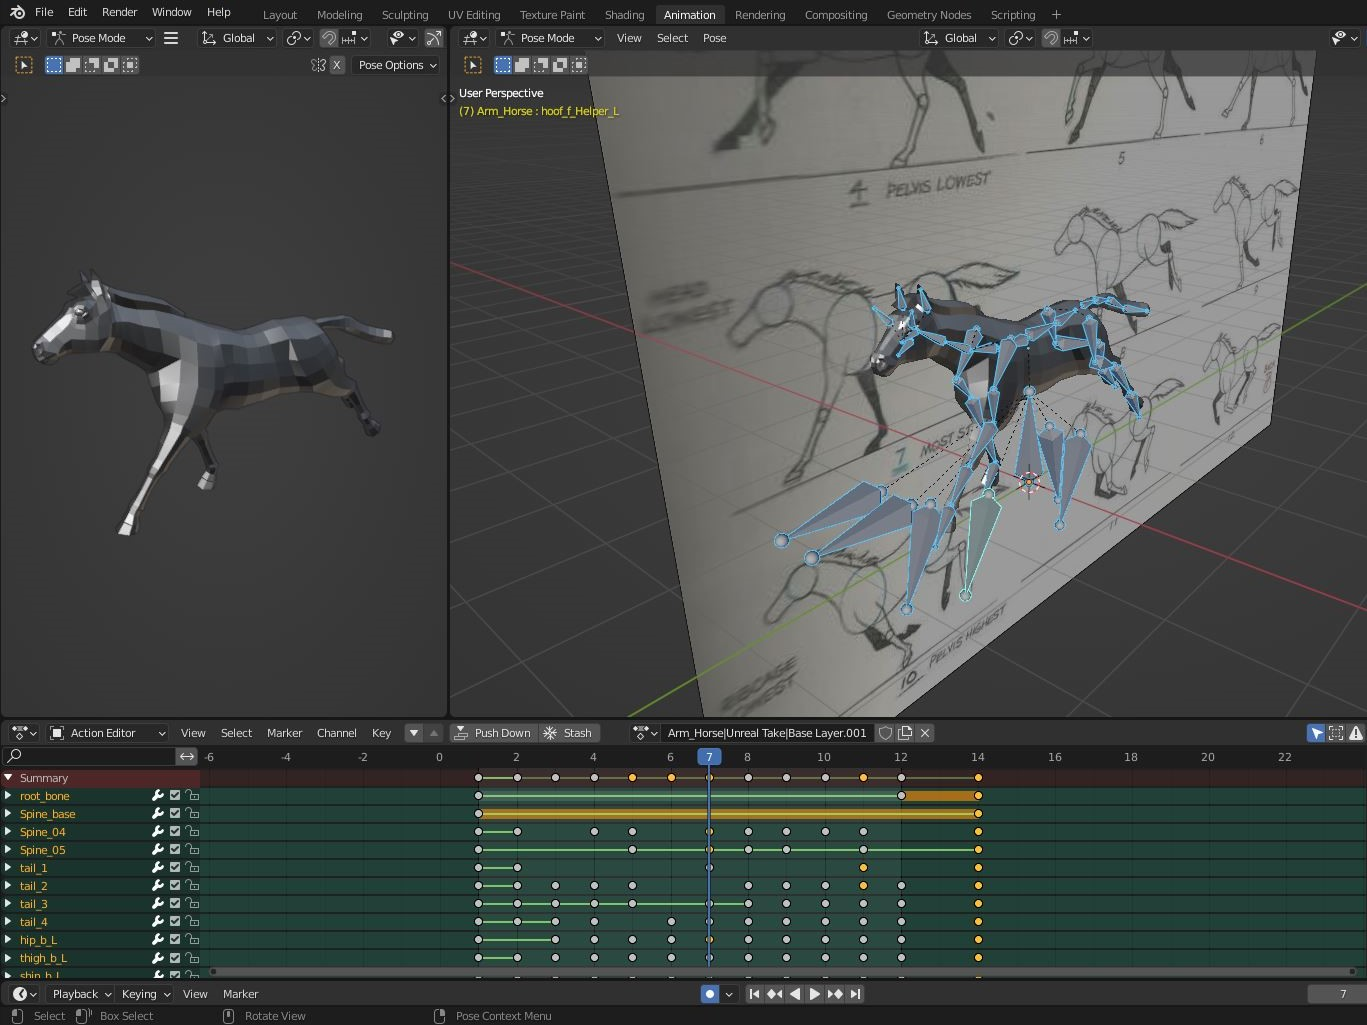
\includegraphics[height=6.5cm]{figure/PoseMode2.JPG}
        \caption{Schermata in cui è possibile vedere la Pose Mode di Blender, l'Action Editor con le keyframe, la mesh del cavallo in una pose con il suo scheletro e l'immagine utilizzata come reference.}
    \end{figure}
    
    \section{Progettazione del mondo 3D}

    Uno degli elementi più importanti quando si parla della costruzione di un mondo immersivo è la creazione del livello 3D.
    %
    Per costruire il livello di gioco sono state utilizzate diverse tecniche offerte dal motore grafico Unreal Engine ma sono stati utilizzati anche degli strumenti offerti dalla suite 3D Blender.
    %
    Unreal Engine infatti permettete di riempire il livello di oggetti con varie tecniche diverse ma questi oggetti devono inizialmente essere creati da un software di modellazione come Blender oppure importati da un asset del marketplace.

    \subsection{I modelli 3D}

    La suite Blender, oltre che per la creazione dell'animazione del galoppo, è stata usata per creare le mesh per questo progetto.
    %
    È stata scelta questa suite per via della sua natura multipiattaforma e per la leggerezza di utilizzo.
    %
    Questo software è stato utilizzato per creare delle mesh interamente e per modificare asset di gioco già esistenti.  

    Infatti, Blender permette di creare Mesh poligonali a partire da figure elementari, queste figure sono: il piano, il cubo, il cerchio, la UV sfera, la ICO sfera, il cilindro, il cono e l'anello.
    %
    Inoltre permette di partire anche da due modelli più complessi: la griglia e la scimmietta Suzanne caratteristica di Blender. 
    %
    Questa scimmietta ha fatto la sua comparsa nel 2002, quando l'azienda fondata da Ton Roosendaal, la \textit{NaN}, era ormai destinata alla bancarotta.
    %
    Gli sviluppatori, in vista dell'inevitabile discontinuità del software, fecero uscire un aggiornamento poco prima della definitiva chiusura che, come piccolo personale tocco, includeva questo Easter Egg.
    %
    Venne chiamata Suzanne come la scimmia del film \textit{Jay and Silent Bob... Fermate Hollywood!}
    %
    Da quel momento Suzanne divenne l'alternativa utilizzabile in Blender come modello di test, oltre ai più comuni Utah Teapot e Stanford Bunny,  per provare materiali, texture ed altro.

    Generalmente, le mesh sono costituite da tre elementi di base: vertici, facce e spigoli. 
    %
    Blender permette di modificare la mesh agendo direttamente su questi elementi utilizzando la Edit Mode.    
    %
    Le mesh create per Metarace con il software Blender sono state: il terreno di gioco, la griglia di start, gli spalti e altri oggetti di gioco come la stalla per i cavalli, una fontana e un campo ippico per la disciplina degli attacchi.
    
    \begin{figure}[!ht] 
        \begin{center}
        \begin{tabular}{c @{\hspace{1em}} c}
        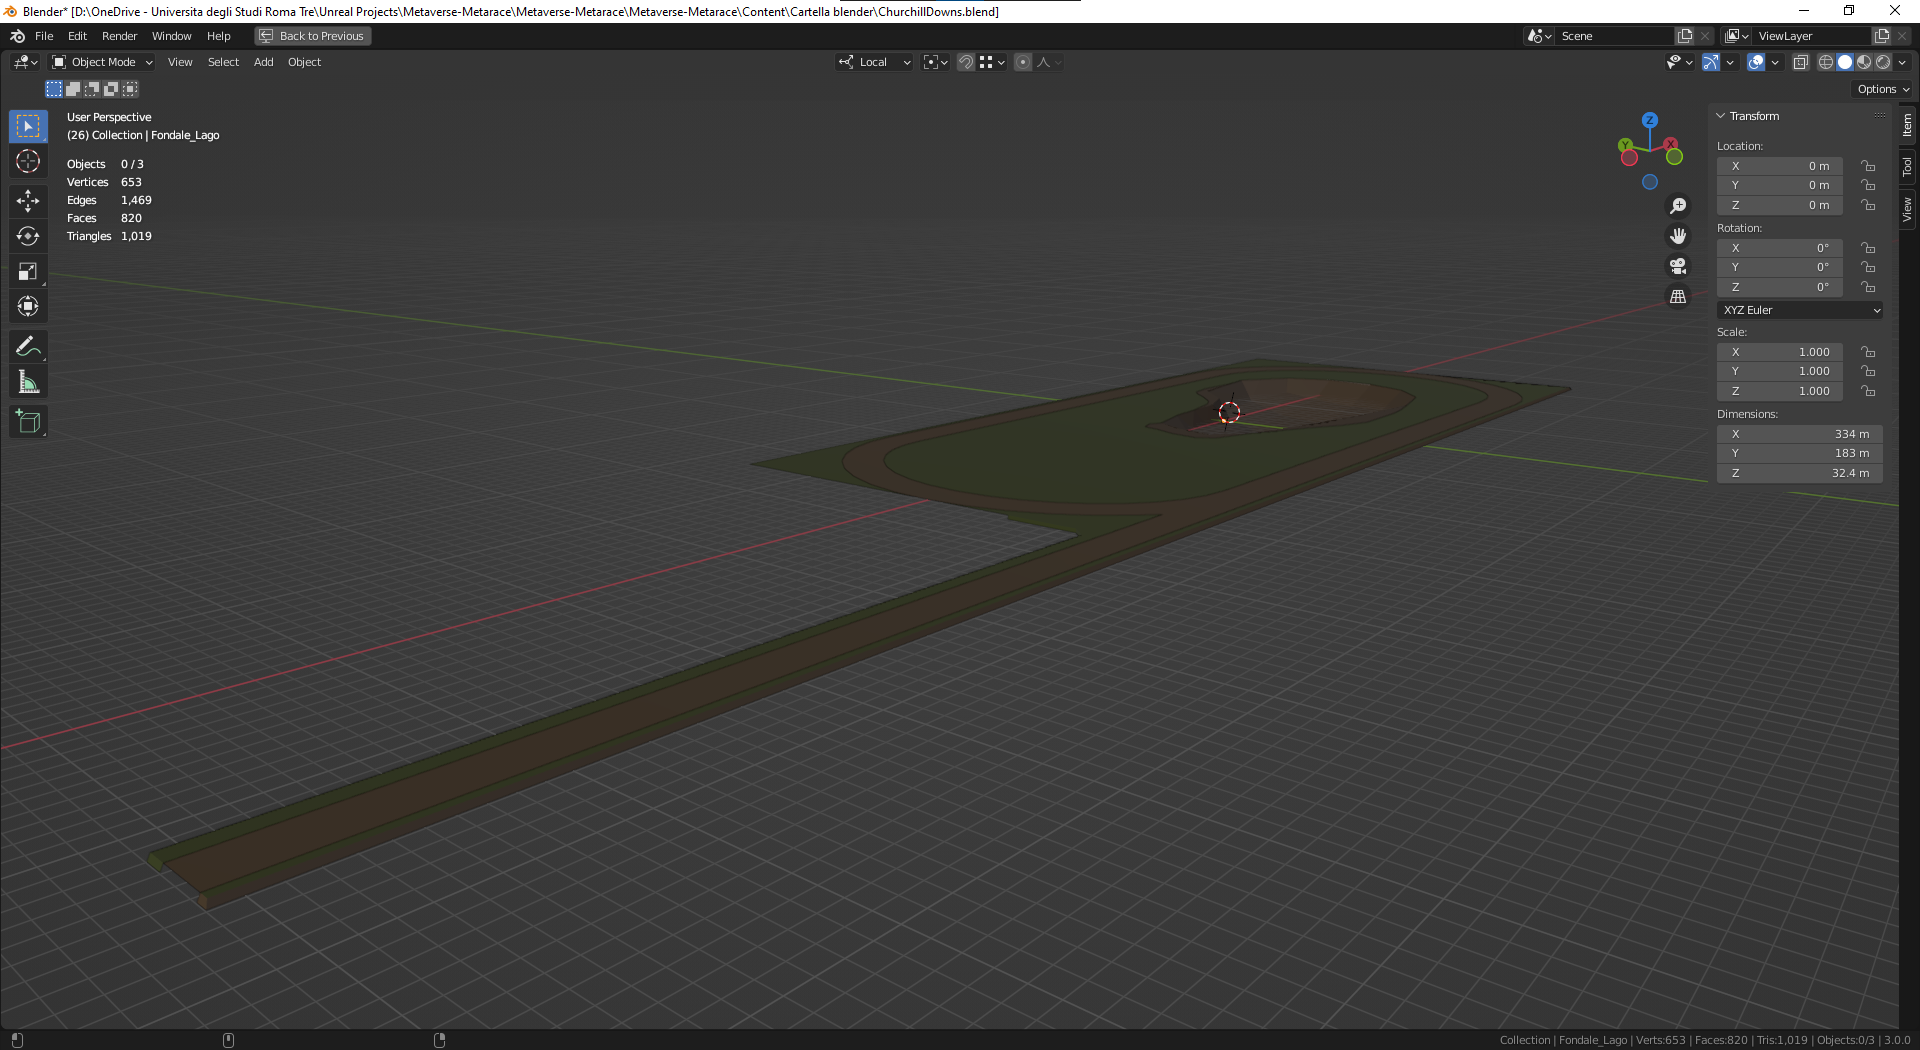
\includegraphics[width=6.5cm]{figure/TerrenoDiGioco.png} &
        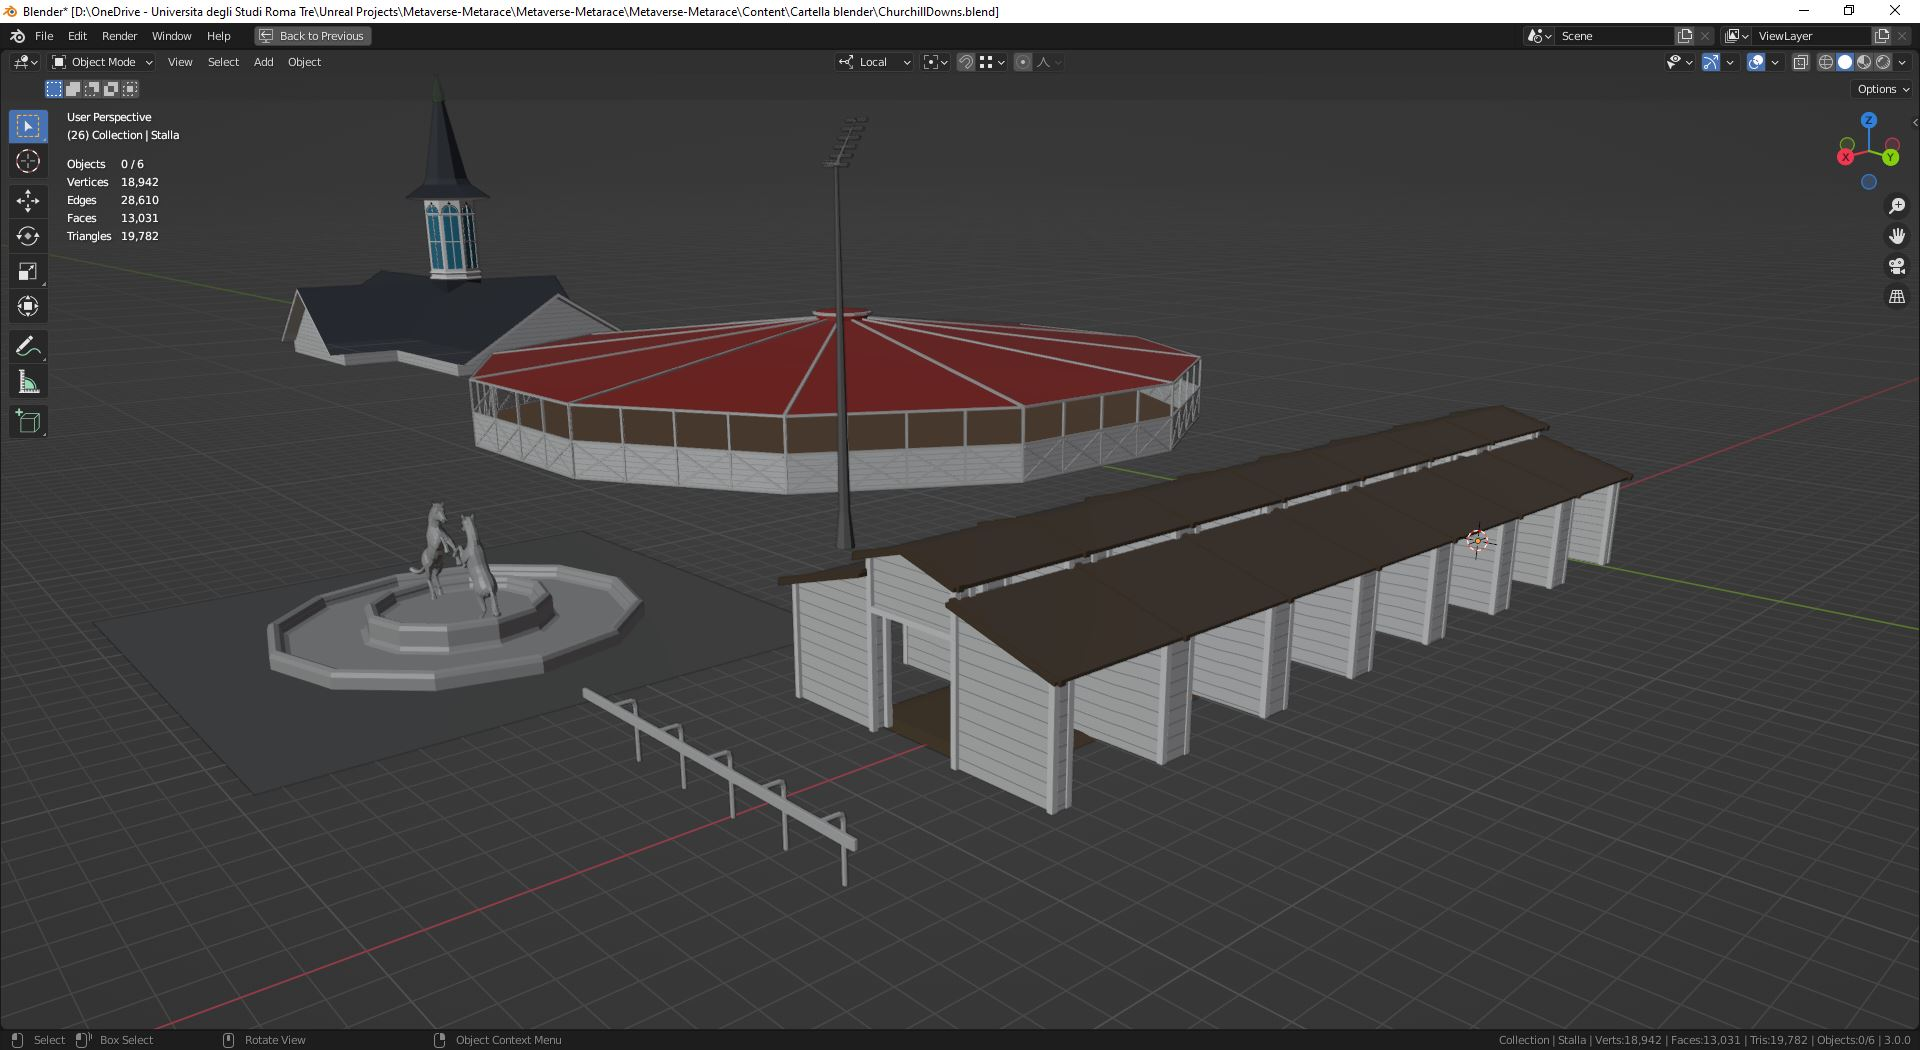
\includegraphics[width=6.5cm]{figure/BlenderModels.JPG} \\
         (a) & (b)
        \end{tabular}
        \end{center}
        \caption{Terreno di gioco in Blender (a) Altri modelli in Blender. (b)}
    \end{figure}

    Queste mesh sono state create in modo da risultare composte da sole facce triangolari.
    %
    Infatti un game engine può usare solo delle mesh con questo tipo di facce.
    %
    È possibile comunque importare su Unreal Engine delle mesh con facce con più lati ma queste verranno automaticamente ricorvertite in triangoli.
    %
    Perciò per evitare distorsioni indesiderate ed errori nella conversione bisogna utilizzare sole facce triangolari oppure facce con al massimo 4 lati che non presentino angoli maggiori di 180°.
    %
    Inoltre maggiore sarà il numero di vertici che una mesh possiede maggiore sarà il carico che il motore di gioco dovrà sopportare per la renderizzazione.
    %
    Per questo motivo le mesh sono state create facendo in modo che il numero dei vertici fosse il più basso possibile.

    Sono state inoltre utilizzate due tecniche di UV mapping (mappatura UV) per la creazione di texture del gioco.
    %
    La mappatura UV è una tecnica che permette di proiettare una o più texture 2D su di un oggetto 3D.
    %
    Le lettere U e V fanno riferimento ai due assi dell'immagine 2D e vegnono usate al posto di X e Y in quanto queste ultime vengono già utilizzate con riferimento agli assi dell'ambiente 3D.
    %
    Vista la natura low poly del gioco, la tecnica principale per la creazione di texture è stata quella di utilizzare una singola immagine per il maggior numero di elementi.
    %
    È possibile infatti creare una texture estremamente leggera costituita da una palette di colori scelti, fare lo unwrap della texture e ridimensionare le UV islands delle facce condensandole in un unico punto della texture in cui è presente il colore che andrà a riempire le facce corrispondenti.

    \begin{figure}[!ht]
        \centering
        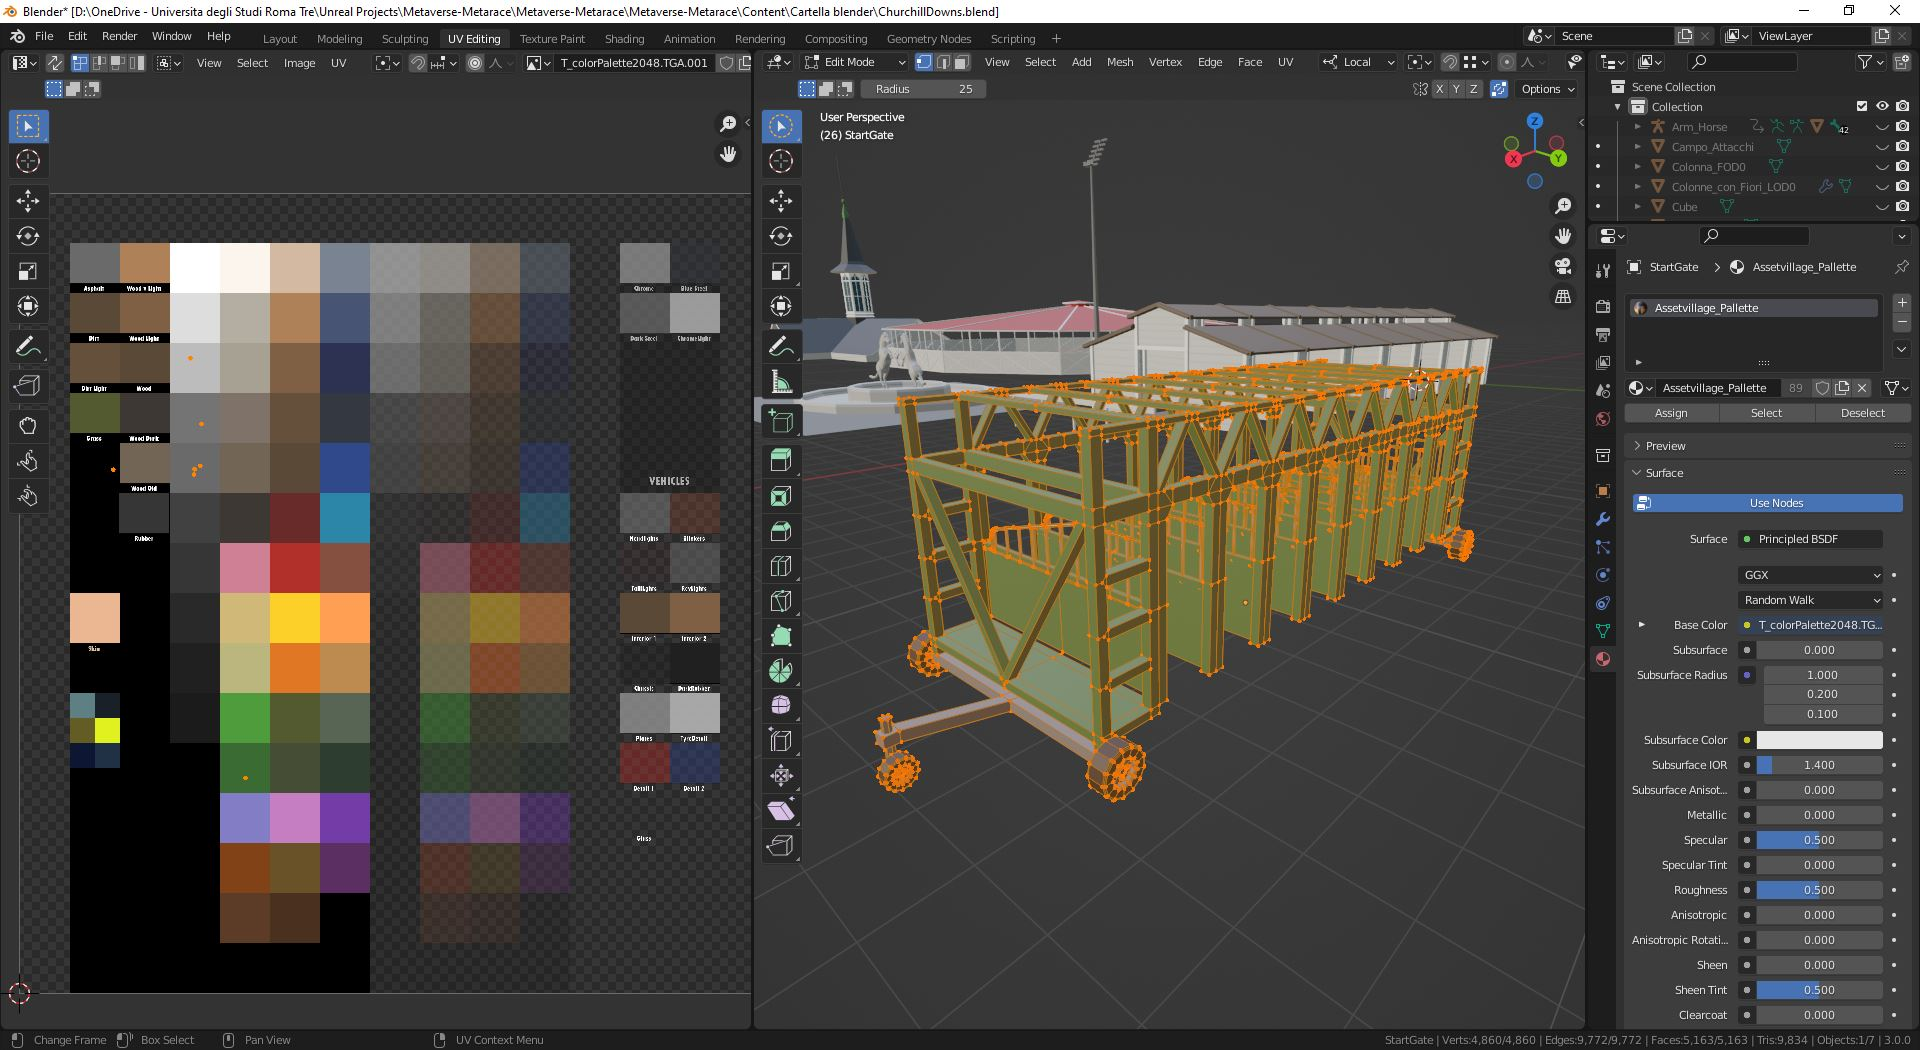
\includegraphics[width=10cm]{figure/BlenderLowPolyTexturing.JPG}
        \caption{Esempio di associazione di UV islands a singoli colori di una sola texture}
    \end{figure}
    
    Questo riduce il numero di istanze di materiali diversi che dovranno esserci nel gioco sia la complessità nel creare le texture stesse e il relativo UVMapping.

    Questa tecnica è una semplificazione della più classica tecnica di mappatura UV dove le UV islands vengono direttamente posizionate sopra la texture in modo che ad ogni faccia corrisponda una particolare zona della texture.
    %
    Il vantaggio di questa tecnica è che è possibile aggiungere della complessità visiva ad una faccia senza aggiungere complessità geometrica.
    %
    Ad esempio per alcuni oggetti di gioco in cui le facce hanno dei pannelli di legno o dei mattoni quelle sono texture assegnate con la tecnica della mappatura UV classica.

    \begin{figure}[!ht]
        \centering
        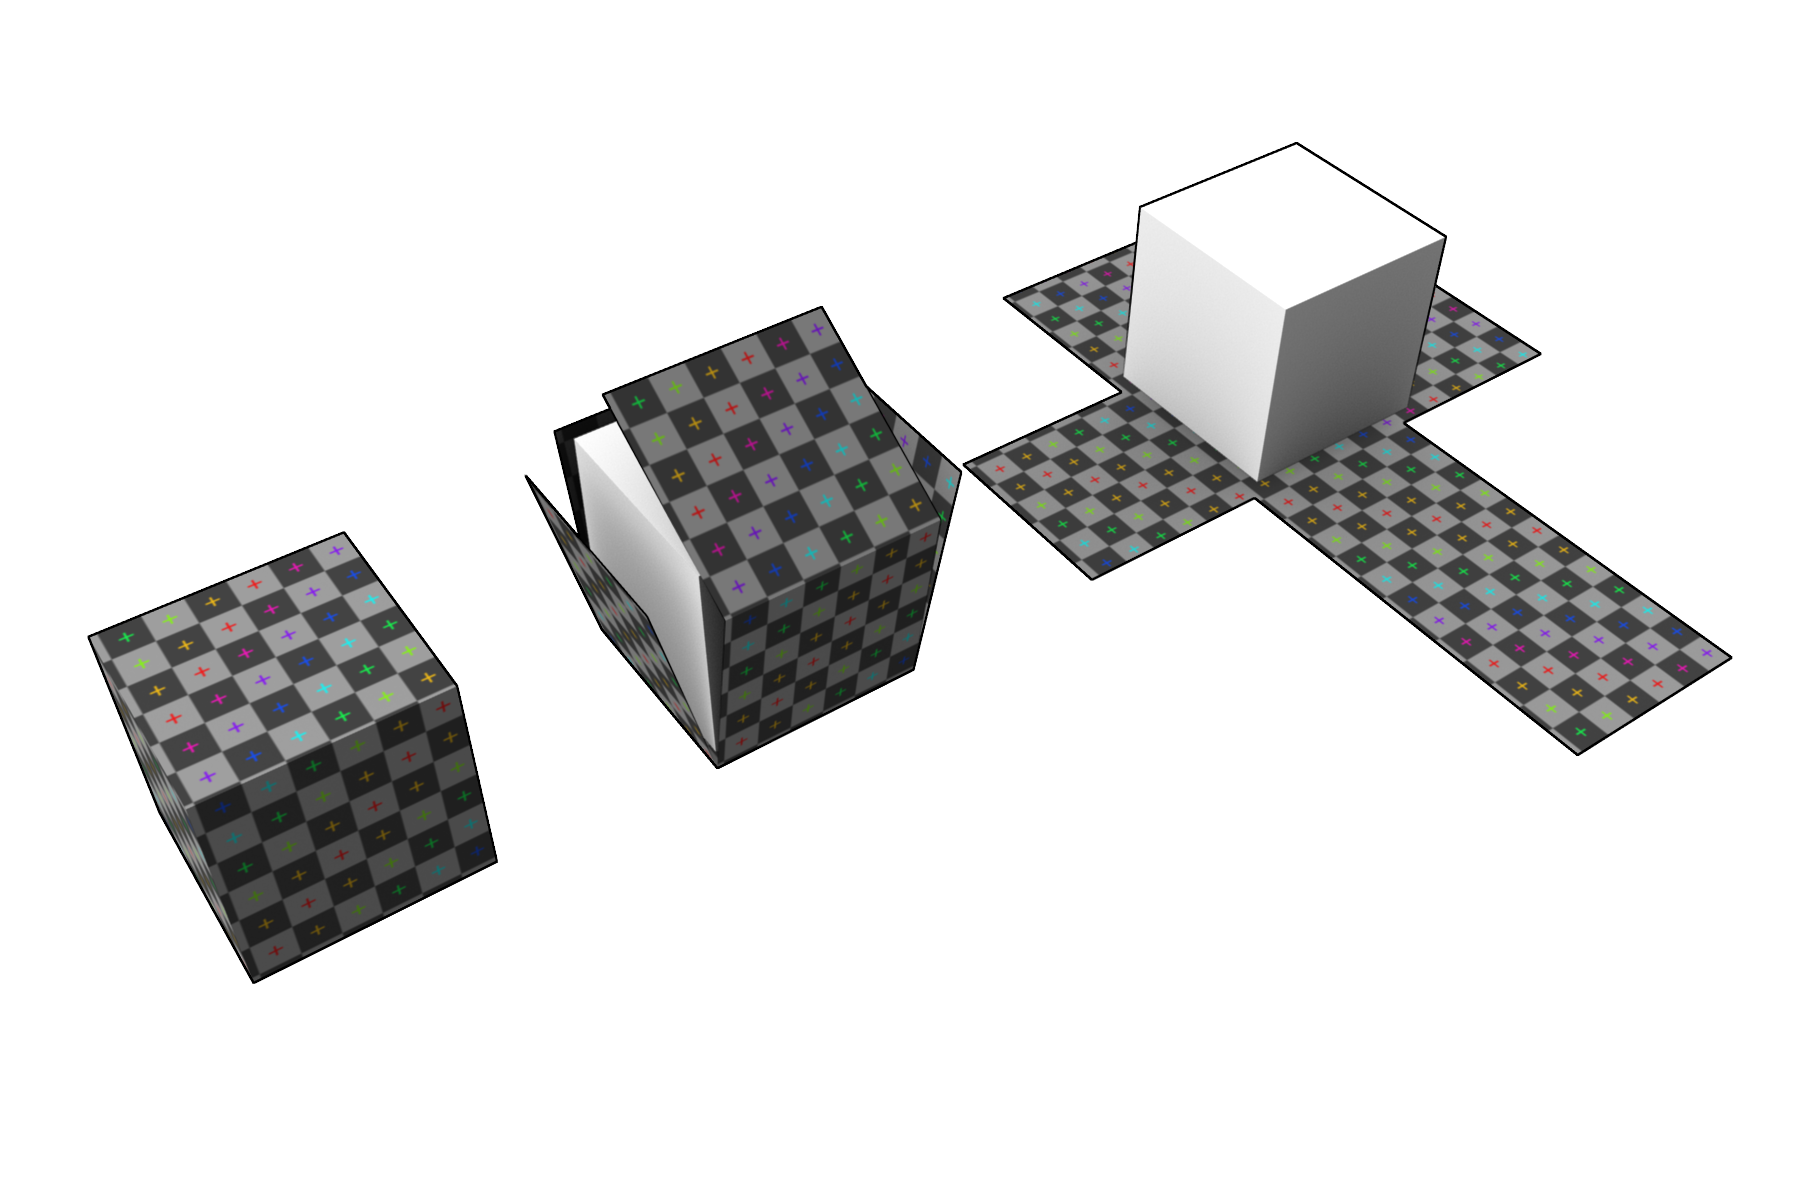
\includegraphics[width=6cm]{figure/UVUnwrapping.png}
        \caption{Schema di funzionamento dell'unwrapping \cite{UVMapsWiki}}
    \end{figure}

    \subsection{Strumenti forniti da Unreal Engine}

    Una volta create le mesh, queste sono state importate all'interno di Unreal Engine.
    
    Una delle tecniche utilizzate per comporre il livello di gioco è stata quella di utilizzare oggetti modulari.
    %
    Ossia oggetti composti da un insieme di mesh statiche che unite insieme possono creare combinazioni anche molto diverse tra loro.
    %
    Questa tecnica ha il vantaggio di ridurre il numero di asset di gioco utilizzati senza perdere l'unicità degli ambienti che è possibile creare.
    %
    Tutti gli edifici in scena sono stati creati utilizzando questa tecnica.
    
    \begin{figure}[t]
        \centering
        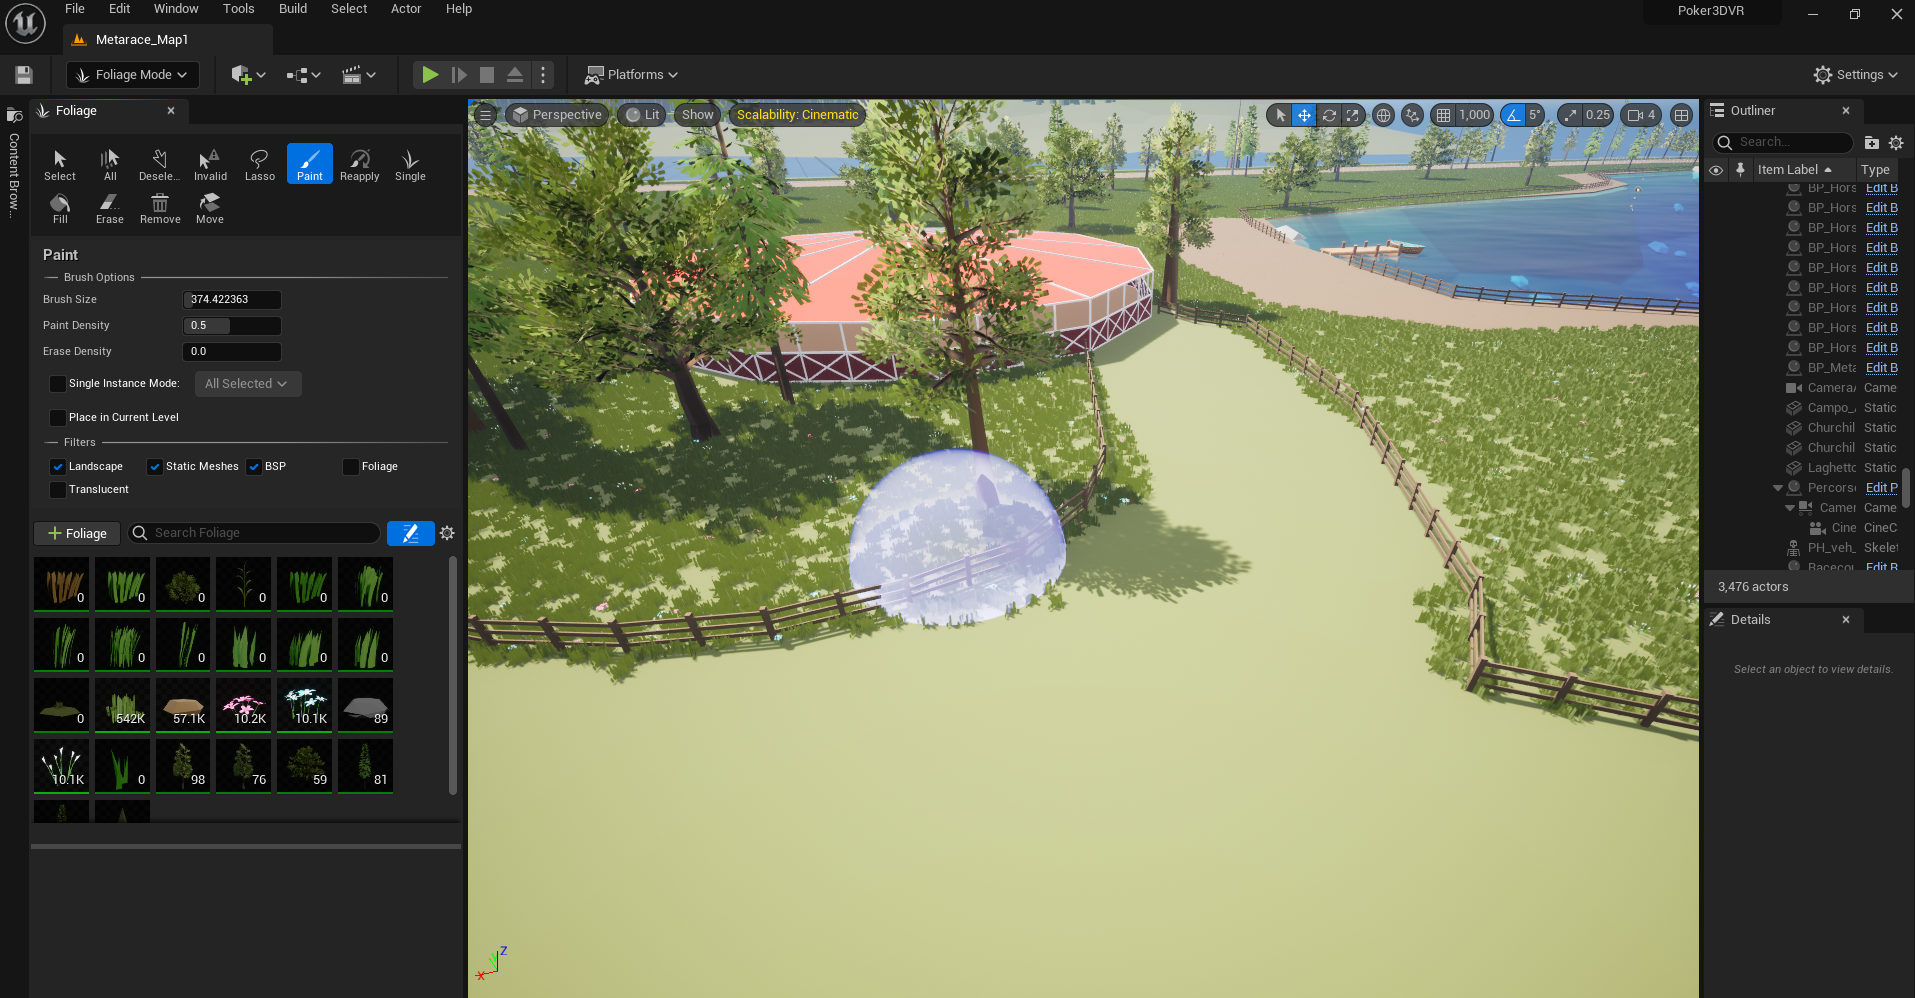
\includegraphics[height= 7cm]{figure/UnrealEngine5Editor.png}
        \caption{Utilizzo del Foliage Tools in Unreal Engine}
    \end{figure}

    Inoltre Unreal Engine permette di aggiungere mesh di gioco in maniera rapida grazie al Foliage Tools.
    %
    Come detto in \ref{sec:Unreal}, è possibile accede alla Foliage Mode tramite il menu delle modalità.
    %
    Questo strumento permette di renderizzare Static Mesh o Actor Foliage sulla superficie di altre geometrie per usarle come effetto di copertura del terreno.
    %
    Tutta la natura presente in Metarace è stata distribuita nel mondo di gioco con questo strumento.

    Un'altro strumento utilizzato è stato il Landscape Tools per la generazione di terreno.
    %
    Per creare scenari molto grandi è meglio utilizzare questa tecnica piuttosto che le Static Mesh perché utilizza solo 4 bytes per i dati di ciascun vertice.
    %
    Le Static Meshes utilizzano invece 12 byte per vertice, più i dati per le tangenti X e Z per ogni faccia racchiuse in 4 byte ciascuno più  da 16 a 32 bit per i dati UV per un totale di 24 o 28 byte a vertice \cite{ULandscape}.
    %
    Inoltre questo strumento fornisce una serie di implementazioni atte ad aumentare l'ottimizzazione del rendering.
    %
    Infatti il sistema di Landscape salva i dati di render del terreno nella memoria dedicata della scheda grafica sotto forma di texture, oltre che supportare il caricaemento delle zone distanti del landscape in LOD (Level Of Details) via via meno complessi geometricamente.

    \begin{figure}[!ht]
        \centering
        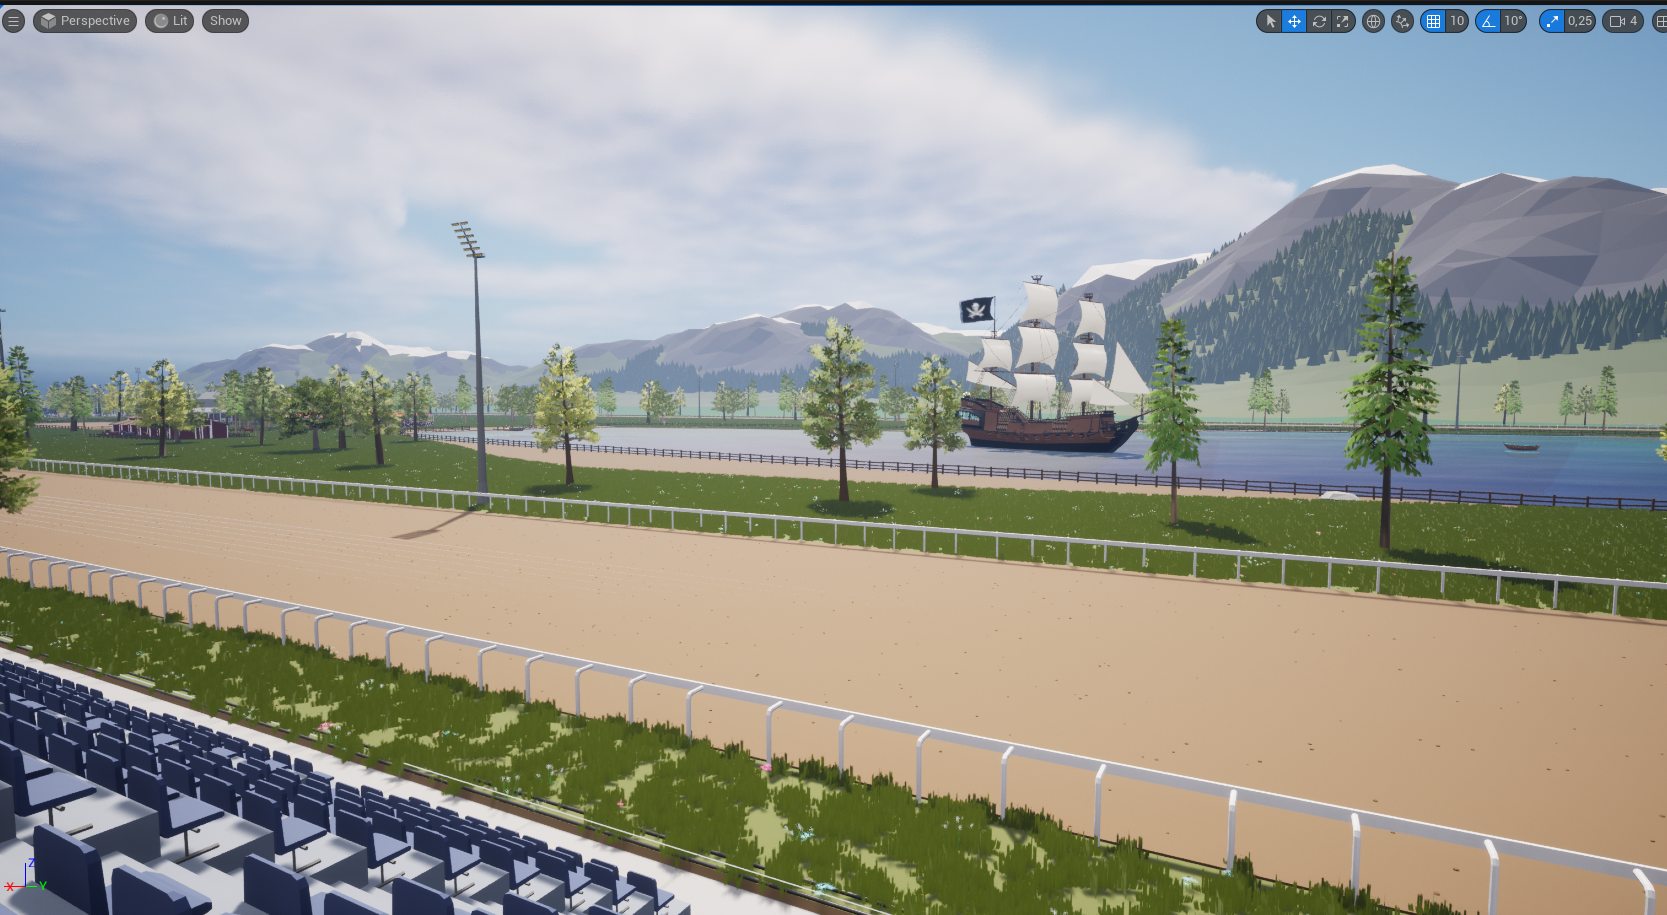
\includegraphics[height=7.5cm]{figure/NaveDaSpaltiCropped.png}
        \caption{Schermata che riprende la vista dagli spalti del percorso}
    \end{figure}
    

    %\section{Analisi del software}

    %\subsection{Modello degli eventi}

% Creare una storia

% Problema e vista storica. Tutto il background storico tecnologico 